\section{Background}
\label{sec:background}

\subsection{Reservoir Computing}

Artificial Neural Networks (ANNs) are a commonly used computational model in machine learning and bio-inspired computing.
Simple, feed forward ANNs lend themselves well to problems were data can be spatially correlated, such as classification.
Many real world problems however, are temporal in nature.
Recurrent neural networks (RNNs) have been shown to be powerful tools for solving temporal problems such as stock market prediction~\cite{Lawrence2001}, learning context free/sensitive languages~\cite{Gers2001} and speech synthesis~\cite{Wu2016}.
Training RNNs is computationally expensive and often requires application specific adaptions of generalized training algorithms in order to reliably converge~\cite{Hammer2002}.
Several techniques have been proposed that circumvent problems related to training, such as Echo State Networks~\cite{Jaeger2001} (ESNs), Liquid State Machines~\cite{Maass2002} (LSMs) and Backpropagation Decorrelation learning~\cite{Steil2004}.
These all share the common feature of only training weights of the output layer of the network, while leaving the hidden layers of the network untrained or simply subject to weight scaling.
In~\cite{Verstraeten2007}, Verstraeten et al.\ propose that systems based on this idea should be unified under the term reservoir computing (RC).

In general, reservoir computing as a term describes any computational system where a dynamic reservoir is excited by input data and output is generated by performing classification/regression over reservoir state.
With its origins in research on various types of recurrent neural networks and training thereof, the reservoir in RC systems is often represented as an RNN.~\cite{Verstraeten2007}
However, any dynamic system capable of eventually forgetting past perturbations and of responding distinctly to different perturbations, can in principle be used.
Snyder et al.~\cite{Snyder2013} investigate using Random Boolean Networks, Yilmaz uses Cellular Automata~\cite{Yilmaz2014} and Fernando et al.\ use a bucket of water~\cite{Fernando2003}.
Figure~\ref{fig:rc-system} shows the basic architecture of any reservoir computing system.


\begin{figure}
  \centering
  \begin{tikzpicture}[auto, node distance=2cm,>=latex']
    \node [block] (input) {Input};
    \node [block, right of=input] (reservoir) {Reservoir};
    \node [block, right of=reservoir] (readout) {Readout};
    \node [block, below of=reservoir] (f) {$f(x)$};
    \node [output, right of=readout] (output) {};

    \draw [->] (input) -- (reservoir);
    \draw [->] (reservoir) -- (readout);
    \draw [->] (readout) -- node [name=out] {Output} (output);
    \draw [->] (out) |- (f);
    \draw [->] (f) -- (reservoir);
  \end{tikzpicture}
  \caption{Basic overview of an RC system.}
\label{fig:rc-system}
\end{figure}

\subsection{Cellular Automata}

John von Neumann introduced cellular automata as a discrete computational model based on local interaction of cells on a grid of finite dimensionality. \todo{citation}
At any timestep $t$ during the simulation, each cell in the grid is in one of a finite number of states.
The state of any cell at time $t+1$ is computed as a function of the cells and its neighboring cells current states.



\subsection{Spiking Neural Networks}

Neural networks can be grouped into three generations, based on the characteristics of their base computational unit, the neuron.
The first generation, based on McCulloch-Pitts neurons, simple threshold gates, allows for universal computation on digital input/output values.
In the second generation, neurons apply a non-linear, continuous activation function on the weighted sum of their inputs.

The third generation of networks bases itself on spiking neurons, which model the interaction between biological neurons more closely.
In this model, a neuron $v$ fires when its potential $P_v$ exceeds a threshold $\theta_v$.
The potential is, at any time, the sum of the postsynaptic potentials, resulting from firing of presynaptic neurons.
The contribution of a spike from presynaptic neuron $u$ at time $s$ to the potential $P_v$ of postsynaptic neuron $v$ is given by $w_{u,v} \cdot \varepsilon_{u,v}(t-s)$, where $w_{u,v}$ is a weight representing the strength of the synapse connecting $u$ and $v$, and $\epsilon_{u,v}(t-s)$ models the response of the spike as a function of time passed since the spike occurred.
A synapse can be both excitatory and inhibitory, meaning that its contribution to the total potential $P_v$ can be both positive and negative.
A biologically plausible response function is shown in figure~\ref{fig:rc-system}.
From a machine learning perspective, the trainable part of a spiking neural network, is the weight $w_{u,v}$, determining to what degree spikes from a neuron $u$ influences the potential of neuron $v$.


In~\cite{Maass1997}, Maass shows that spiking neurons are at least computationally equal to the models used in generation one and two, and that they can also be more efficient in terms of neurons required to compute a function.
SNNs also have the required attributes to be used as a reservoir in an RC system.~\cite{Pipa2010}
\todo{elaborate?}

\begin{figure}
  \centering
  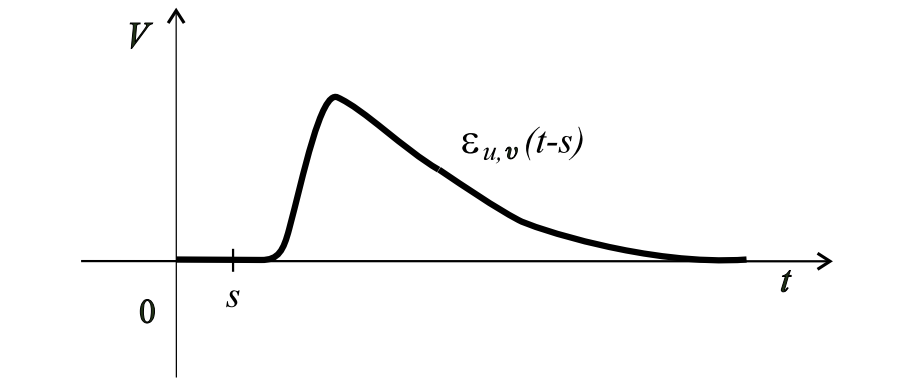
\includegraphics[width=\linewidth]{figures/response-function-snn}
  \caption{Common spike response function shape}
\label{fig:response-function-snn}
\end{figure}
